Due to the fact that the project team is composed of several developers, who
must review and integrate their work together, it has been necessary to
establish a set of common coding standards.

In addition, because of the software-free character of the project, the code is
public, and throughout its life will be maintained by multiple developers. For
this reason, a great effort had to be dedicated to ensuring the readability of
the code, along with its documentation, and compliance with strictly established
standards. Among these standards are included two Python Enhancements Proposals
(PEPs), which are the directives that set the different conventions in Python:
the PEP 8 - Style Guide for Python Code, and the PEP 257 -Docstring Conventions.

PEP 257 documents the semantics and conventions associated with Python
docstrings, which allow include documentation within the code. These docstring
are found next to the code as headers of modules, classes or functions. It has
been used a google-like docstring style, based in the reStructuredText format.
This style allows the automatic generation of documentation in pdf and html,
using the Sphinx tool. These pages generated automatically are maintained by
the continuous integration system and may be consulted online on
https://fda.readthedocs.io/.

\begin{figure}[Scikit-fda online documentation]{FIG:AMPPHA}{Scikit-fda online documentation}
  \subfigure[SBFIG:DOC]{Documentation of function}{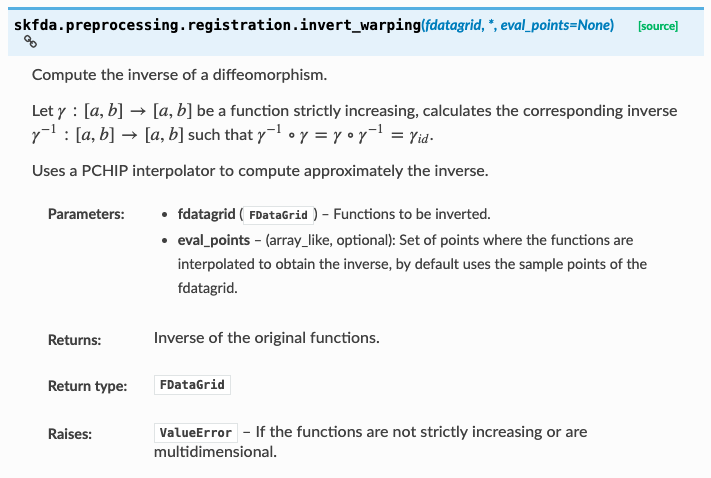
\includegraphics[width=7cm]{doc-a}} \quad
  \subfigure[SBFIG:DOCTEST]{Doctest included within the documentation}{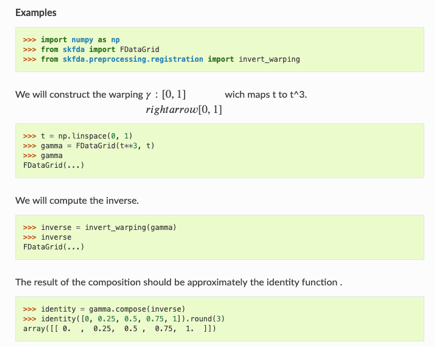
\includegraphics[width=7cm]{doc-b}}
\end{figure}

In addition, among the advantages of this kind of documentation is the
possibility of including examples embedded in it, called doctests, which appears
 as dynamic short examples within de documentation, as it is shown in the
 figure \ref{SBFIG:DOCTEST}.

These examples are in turn tests. When running the bench tests, using the tool
pytest, the code is parsed looking for doctests, executing the code found in
them and checking that the output matches with the output of the documentation.

However, the fundamental part of the testing is made up of unit tests, which are
executed together with the doctests to check the integrity of the software.

A very relevant part of the package documentation is made up of examples,
which are Python notebooks written as tutorials. Due to their extension, these
examples can be found in Annex C or among the online documentation. Below it is
shown the beginning of one of these examples.

\textbf{HERE WILL BE AN EXAMPLE.}
